\documentclass[aspectratio=169]{beamer}

\mode<presentation>
\usetheme{Boadilla}
\definecolor{redback}{RGB}{140,0,0}
\definecolor{blue}{RGB}{30,90,205}
\definecolor{red}{RGB}{213,94,0}
\definecolor{green}{RGB}{0,128,0}
\setbeamercolor{title}{fg=redback}
\setbeamercolor{frametitle}{fg=redback}
\setbeamercolor{block title}{bg=redback, fg=white}
\setbeamercolor{block body}{bg=white}
\setbeamercolor{structure}{fg=redback}
\setbeamercolor{item projected}{fg=white}
\setbeamercolor{item}{fg=redback}
\setbeamercolor{subitem}{fg=redback}
\setbeamercolor{section in toc}{fg=redback}
\setbeamercolor{description item}{fg=redback}
\setbeamercolor{caption name}{fg=redback}
\setbeamercolor{button}{bg=redback, fg=white}
\setbeamercolor{caption name}{fg=redback}
\usepackage{graphics}
\usepackage{tikz}
\usepackage{amsmath}
\usepackage{bbm}
\usetikzlibrary{decorations.pathreplacing}
\usepackage{geometry}
\usepackage{booktabs}
\usepackage{multirow, makecell}
\usepackage{float}
\usepackage{fancyvrb}
\usepackage{kotex}
\usepackage{caption}
\usepackage{subcaption}
\usepackage{adjustbox}
\usepackage{hyperref}
\usepackage{threeparttable}
\usepackage[scaled=0.92]{helvet}
\usepackage[default]{lato} %If I want a twist
\newenvironment{wideitemize}{\itemize\addtolength{\itemsep}{10pt}}{\enditemize}
\newenvironment{wideenumerate}{\enumerate\addtolength{\itemsep}{10pt}}{\endenumerate}
\newenvironment{widedescription}{\description\addtolength{\itemsep}{10pt}}{\enddescription}
\hypersetup{
colorlinks=true,
linkcolor=redback,
filecolor=green, 
urlcolor=blue,
}
\beamertemplatenavigationsymbolsempty
\setbeamercolor{author in head/foot}{bg=white, fg=redback}
\setbeamercolor{title in head/foot}{bg=white, fg=redback}
\setbeamercolor{date in head/foot}{bg=white, fg=redback}
\setbeamercolor{section in head/foot}{bg=white, fg=redback}
\setbeamercolor{page number in head/foot}{bg=white, fg=redback}
\setbeamercolor{headline}{bg=redback}
\setbeamertemplate{footline}{
    \leavevmode%
    \hbox{%
        \begin{beamercolorbox}[wd=.333333\paperwidth,ht=2.25ex,dp=1ex,center]{date in head/foot}%
            \usebeamerfont{date in head/foot}\insertshortdate
        \end{beamercolorbox}%
        \begin{beamercolorbox}[wd=.444444\paperwidth,ht=2.25ex,dp=1ex,center]{title in head/foot}%
            \usebeamerfont{title in head/foot}\insertshorttitle
        \end{beamercolorbox}%
        \begin{beamercolorbox}[wd=.222222\paperwidth,ht=2.25ex,dp=1ex,center]{page number in head/foot}%
            \usebeamerfont{page number in head/foot} \insertframenumber{} / \inserttotalframenumber
        \end{beamercolorbox}}%
        \vskip0pt%
    }

\setbeamertemplate{section in toc}[sections numbered]
\setbeamertemplate{subsection in toc}{\leavevmode\leftskip=3em\rlap{\hskip-1.75em\inserttocsectionnumber.\inserttocsubsectionnumber}\inserttocsubsection\par}
\setbeamerfont{subsection in toc}{size=\footnotesize}

\newenvironment{transitionframe}{\setbeamercolor{background canvas}{bg=redback}\setbeamertemplate{footline}{} \begin{frame}}{\end{frame}}
\newcommand{\ROM}[1]
    {\MakeUppercase{\romannumeral #1}}
    \DeclareMathOperator*{\plim}{plim}
\makeatletter
\let\@@magyar@captionfix\relax
\makeatother


\title[Recitation 11 (Intro to Econometrics \ROM{2})]{Recitation 11: DiD and IV approaches to Treatment Effects} % Change this regularly
\author[]{Seung-hun Lee }
\institute[]{Columbia University \\ Introduction to Econometrics \ROM{2} Recitation}

\date[April 18th, 2022]{April 18th, 2022}

\begin{document}
\begin{frame}
\titlepage
\end{frame}


%%% Color slides for section headers: Use for colloquium version (The ones bewteen \iffals and \fi)

\begin{transitionframe}
  \begin{center}
         { \Huge \textcolor{white}{Difference-in-Difference estimation}}
       \end{center}
\end{transitionframe}

\begin{frame}
\frametitle{Simple DiD regression: 2 Groups and 2 periods}
\begin{itemize}
\item  `Before and after' ($t_0$ and $t_1$) and treated vs untreated ($G_i=1$ and $G_i=0$)
\item No one treated at $t_0$ but $G_i=1$ group is treated at $t_1$, $G_i=0$ are never treated 
\item We can define a treatment framework as
\[
y_{i,t}=G_iy_{i}(1,t)+(1-G_i)y_{i}(0,t) \ \ (t\in\{t_0, t_1\})
\]
\item What we observe: $(y_{i,t_1}, y_{i,t_0},G_i, X_i)$ for every unit $i$
\item What we do not: $y_i(1,t_1)$ for those in $G_i=0$ and $y_i(0,t_1)$ for those in $G_i=1$
\end{itemize}
\end{frame}

\begin{frame}
\frametitle{Parallel trend is a CIA assumption in this setup}
\begin{itemize}
\item We define it as 
\[
(y_i(1,t_1)-y_i(1,t_0), y_i(0,t_1)-y_i(0,t_0)) \perp\!\!\! \perp G_i|X_i
\]
Or we can let $y_i(G_i,t_0)=y_i(t_0)$ for $G_i\in\{0,1\}$ since no one is treated then and write
\[
(y_i(1,t_1)-y_i(t_0), y_i(0,t_1)-y_i(t_0)) \perp\!\!\! \perp G_i|X_i
\]
\item Changes in treatment outcome for both groups are independent of $G_i$ with $X_i$ controlled for
\begin{itemize}
\item Violated if uncontrolled factors affect the changes in the outcome or if there are differences in the trends of $y_{i,t}$ across treated and control groups before the experiment.
\end{itemize}
\end{itemize}
\end{frame}


\begin{frame}
\frametitle{Parallel trend is a CIA assumption in this setup}
\begin{itemize}
\item Let $D_i=G_i$ and write
\begin{align*}
y_i = y_{i,t_1}-y_{i,t_0}&=D_i(\underbrace{y_i(1,t_1)-y_i(1,t_0)}_{y_i(1)})+(1-D_i)(\underbrace{y_i(0,t_1)-y_i(0,t_0)}_{y_i(0)})\\
&=D_iy_i(1) + (1-D_i)y_i(0)
\end{align*}
Thus, we can write $(y_i(1), y_i(0)) \perp\!\!\! \perp D_i|X_i$
\item Testing for this is technically not feasible
\begin{itemize}
\item As a close approach: Select a time period $\tilde{t}<t_0$ and find out if the difference $y_i(t_0)-y_i(\tilde{t})$ is independent with $G_i$
\item Do this by plotting  pre-treatment outcome (not perfect: does not perfectly take into account the influence of unobserved factors)
\item If nonzero difference/pre-trends observed: Sure sign of nonparallel trends
\end{itemize}
\end{itemize}
\end{frame}


\begin{frame}
\frametitle{Not to difficult to implement}
\begin{itemize}
\item We can write
\[
y_{it}=\beta_0(X_i)+\beta_1(X_i)\cdot\mathbb{I}[t=t_1]+\beta_2(X_i)\cdot G_i + \beta_3(X_i)\cdot G_i\cdot\mathbb{I}[t=t_1]+\epsilon_{it}
\]
\item In this context, the treatment effect for $X_i=x$ would be
\begin{align*}
TE(x)&=E[y_i(1)-y_i(0)|X_i=x]\\
&=E[(y_i(1,t_1)-y_i(1,t_0))-(y_i(0,t_1)-y_i(0,t_0))|X_i=x]\\
&=x\cdot E[\{(\beta_0+\beta_1+\beta_2+\beta_3)-(\beta_0+\beta_2)\}-\{(\beta_0+\beta_1)-(\beta_0)\}|X_i=x]\\
&=x\cdot E[(\beta_1+\beta_3)-\beta_1|X_i=x]\\
&=\beta_3 x
\end{align*}
So $\beta_3$ would be our parameter of interest.
\end{itemize}
\end{frame}

\begin{frame}
\frametitle{Extending to TWFE}
\begin{itemize}
\item in $2\times2$ setup, DiD is equivalent to TWFE
\[
y_{it}=a_i+b_t + cD_{it}+e_{it}
\]
where $D_{it}=1$ if unit $i$ is treated at period $t$ and $0$ if otherwise
\item Treatments can be implemented in multiple periods: Let $D_{i\tau}=0$ if $D_{it}=1$ and $\tau>t$
\item New problem: Overall trend in the data is reversed or attenuated relative to a trend that appears in the groups composing the data (Simpson's paradox)
\begin{itemize}
\item In the case where there is a strong heterogeneity of treatment across groups or time, the coefficient of $c$ may be reversed from the true effect
\end{itemize}
\end{itemize}
\end{frame}

\begin{frame}
\frametitle{Treatment effect as an weighted average of $i\times t$ cells}
\begin{itemize}
\item Let $G_i$ be the first period in which $i$ is treated ($G_i=\infty$ if never treated)
\item  By applying (two-step) within estimation, we can get
\[
\hat{c} = \frac{\sum_{i.t}\tilde{y}_{it}\widetilde{D}_{it}}{\sum_{i.t}\widetilde{D}_{it}^2}
\]
\item By FWL, we get the same estimate by regressing $y_{it}$ onto the residual of 
\[
D_{it} = a_i+b_i+u_{it} 
\]
In this way, we can write
\[
\hat{c}=\frac{\sum_{i,t}y_{it}\hat{u}_{it}}{\sum_{i,t}\hat{u}_{it}^2}=\sum_{i,t}y_{it}\left(\frac{\hat{u}_{it}}{\sum_{i,t}\hat{u}_{it}^2}\right)
\]
\end{itemize}
\end{frame}

\begin{frame}
\frametitle{Problematic case: Early-adopters with negative weights at large $t$}
\begin{itemize}
\item Some observations end up getting \textit{negative} weights. 
\begin{itemize}
\item This happens since $\hat{u}_{it}$ is not necessarily binary, and those whose treatment intensity is below the mean gets negative weights.
\item  Early adopters in later years (high unit-level treatment mean and time-level treatment mean) end up with negative weights.  
\end{itemize}
\item Minimum requirement is to vary the coefficient $c$ across different implementation period, $c(G_i)$ (a simple event-study)
\item Not enough: We want to compare the average treatment effect for those treated earlier vs. later. Specifically, for a specific $g\leq t$,  and for any $g'>t$, write
\[
E[y_{it}(g)-y_{it}(\infty)|G_i=g]=E[y_{it}-y_{i,g-1}|G_i=g]-E[y_{it}-y_{i,g-1}|G_i=g']
\]
\item It is nicer to have those who are never treated (pure control)
\end{itemize}
\end{frame}

\begin{transitionframe}
  \begin{center}
         { \Huge \textcolor{white}{Selection on unobservables: Setup and IV approach}}
       \end{center}
\end{transitionframe}




\begin{frame}
\frametitle{Violation of CIA: Selection on unobservables}
\begin{itemize}
\item Even with controls, assignment may fail to be random
\begin{itemize}
\item Participants self-select based on expected benefit: Failure to predict expected benefit with observables
\item Participants may be selected, consciously or not, to join: Participants and nonparticipants systematically differ on something that is not usually observed.
\item There may be equilibrium effects: Outcomes may be subject to spillover effects (Think of control groups that are also inadvertently exposed to treatment)
\end{itemize}
\item Mathematically, we end up with
\small{\begin{align*}
E[y_i|D_i=1,x]-E[y_i|D_i=0.x]&=\mu(x,1)-\mu(x,0)+E[\epsilon_i(1)|D_i=1,x]-E[\epsilon_i(0)|D_i=0,x]\\
&=TE+\underbrace{E[\epsilon_i(1)|D_i=1,x]-E[\epsilon_i(0)|D_i=0,x]}_{\text{(Positive/Negative) selection bias}}
\end{align*}}\normalsize
\begin{itemize}
\item $E[\epsilon(d)|D_i, X_i]$ no longer zero, and $(\epsilon_i(1), \epsilon_i(0))$ and the $u_i$ in $D_i=\mathbb{I}[u_i<p(x_i)]$ can covary
\end{itemize}
\end{itemize}
\end{frame}

\begin{frame}
\frametitle{Old approach: Heckman's two-step estimates}
\begin{itemize}
\item We have a data generating process
\[
y_i = \max\{X_i\beta+\sigma\eta_i, 0\}, \eta_i \sim N(0,1)
\]
So we only see $y_i$ if $X_i\beta+\sigma\eta_i>0$. We are able to observe $D_i$, specified as
\[
D_i=\begin{cases}1 & \text{if }\eta>-\frac{X_i\beta}{\sigma}\\ 0 & \text{otherwise} \end{cases}
\]
\item Then, for the observed sample, we are likely to have an $\eta_i$ that is positively selected
\item Adjust by regressing $D_i$ on $X_i$ to get ($\widehat{\beta/\sigma}$) and include estimate of $\frac{\phi(X_i\beta/\sigma)}{\Phi(X_i\beta/\sigma)}$ into the regression ($y_i = X_i\beta+ \gamma\widehat{\frac{\phi(X_i\beta/\sigma)}{\Phi(X_i\beta/\sigma)}}+\epsilon_i$)
\item Not recommended: If errors are non-normal, incorrect specification
\end{itemize}
\end{frame}


\begin{frame}
\frametitle{IV approach: Relevance, Exclusion, and Monotonic}
\begin{itemize}
\item \textbf{Relevancy}: It effects the propensity score $p(w,z)=\Pr(D_i=1|W_i=w, Z_i=z)$
\item \textbf{Exclusion}: Distribution of the counterfactual outcomes and $u_i$ does not depend on $Z_i|X_i$. To put it in mathematical notation, 
\[
(y_i(1), y_i(0), u_i) \perp \!\!\!\perp Z_i|W_i
\]
\item \textbf{Monotonicity}: For a given $W_i=w$, $z$ changes the treatment in the same direction for everyone. This is also called a no two-way movement condition.
\begin{itemize}
\item Only partially testable: For each $i$, only one of $z$ or $z'$ exists (intuition and proxy based on changes in treatment enrollment after changes in $Z_i$)
\end{itemize}
\end{itemize}
\end{frame}

\begin{frame}
\frametitle{We identify treatment effects on compliers!}
\begin{itemize}
\item Exclusion: $u_i$ and the outcome can be correlated, but the changes in $Z_i$ not affect $u_i$ and outcome conditional on $W_i$
\begin{itemize}
\item In that regard, we need to rewrite our $y_i(d)$ notation as 
\[
y_i(d)=\mu(w,d)+\epsilon_i(d)
\]
\end{itemize}
\item Relevance: By moving from $p(w,z)$ to some larger $p(w,z')$, we find compliers, a group of individuals who do not get treated at $p(w,z)$ but do get treated at $p(x,z')$
\begin{itemize}
\item Also: Always-takers and never-takers
\end{itemize}
\item Monotonicity: Prevents the case where $u_i<p(w,z)$ when $Z_i=z$ but $u_i'>p(x,z')>p(w,z)$ when $Z_i=z'$
\begin{itemize}
\item This groups is referred to as defiers
\item $u_i$ moves with $Z_i$ and in an opposite direction: This violate exclusion as well (and monotonicity is also known as no two-way movement)
\end{itemize}
\end{itemize}
\end{frame}


\begin{frame}
\frametitle{Local average treatment effect: Treatment localized to compliers!}
\begin{itemize}
\item Narrow the interest to compliers, and get average treatment effect on this group
\item Setup
\begin{itemize}
\item Fix $W_i=w$
\item $Z_i$ will be a binary instrumental variable. Think of this as a variable that affects eligibility but not related to outcome 
\item $D_i(w, z)$ can be characterized as $D_i(w, z)=\mathbb{I}[u_i<p(w,z)]$. Note that as $z$ rises, so will $p(w,z)$ due to relevance condition. 
\item $Z_i$ itself has no bearing, at least directly, on the outcome. So $y_i(d)=\mu(w,d)+\epsilon_i(d)$. So we still have $(\epsilon_i(1), \epsilon_i(0), u_i)\perp\!\!\!\perp Z_i|X_i$. 
\end{itemize} 
\item LATE is defined as
\[
LATE(w,z,z')=E[y_i(1)-y_i(0)|p(w,z)<u_i<p(w,z'), W_i=w]
\]
\end{itemize}
\end{frame}

\begin{frame}
\frametitle{Obtaining LATE from the data: Other group ruled out}
\begin{itemize}
\item Breaking down the equation
\footnotesize{\[
\begin{aligned}
E[y_i|X_i=x']-E[y_i|X_i=x]&=E[\mathbb{I}[u_i<p(x')]y_i(1)+\mathbb{I}[u_i>p(x')]y_i(0)|x']\\
&\ \ \ \ -E[\mathbb{I}[u_i<p(x)]y_i(1)+\mathbb{I}[u_i>p(x)]y_i(0)|x]\\ 
&=E[\mathbb{I}[u_i<p(x')]y_i(1)+\mathbb{I}[u_i>p(x')]y_i(0)]\\
&\ \ \ \ -E[\mathbb{I}[u_i<p(x)]y_i(1)+\mathbb{I}[u_i>p(x)]y_i(0)]\ (\because\text{Exclusion})\\
&=E[(\mathbb{I}[u_i<p(x')]-\mathbb{I}[u_i<p(x)])y_i(1)\\
&\ \ \ \ -(\mathbb{I}[u_i>p(x')]-\mathbb{I}[u_i>p(x)])y_i(0)]\\
&=E[(\mathbb{I}[u_i<p(x')]-\mathbb{I}[u_i<p(x)])(y_i(1)-y_i(0))]\\
&=\Pr(\mathbb{I}[u_i<p(x')]-\mathbb{I}[u_i<p(x)]=1)\\
&\ \ \ \ \times E[y_i(1)-y_i(0)|\mathbb{I}[u_i<p(x')]-\mathbb{I}[u_i<p(x)]=1]
\end{aligned}
\]}\normalsize
\item $\mathbb{I}[u_i<p(x')]-\mathbb{I}[u_i<p(x)]=0$ for never-takers and always-takers
\item Defiers ruled out by monotonicity
\end{itemize}
\end{frame}

\begin{frame}
\frametitle{Obtaining LATE from the data: LATE as Wald}
\begin{itemize}
\item As a result, we get 
\begin{gather*}
\Pr(\mathbb{I}[u_i<p(x')]-\mathbb{I}[u_i<p(x)]=1)E[y_i(1)-y_i(0)|\mathbb{I}[u_i<p(x')]-\mathbb{I}[u_i<p(z)]=1]\\
=\Pr(p(x)<u_i<p(x'))E[y_i(1)-y_i(0)|p(x)<u_i<p(x')]
\end{gather*}
\item Therefore, we are able to back out the definition of the LATE and can identify them as
\[
LATE(w, z, z')=\frac{E[y_i|X_i=x']-E[y_i|X_i=x]}{\Pr(p(x)<u_i<p(x'))}=\frac{E[y_i|X_i=x']-E[y_i|X_i=x]}{p(x')-p(x)}
\]
\item We can go further: Estimate propensity scores with $p(w,z)=E[D_i|W_i=w, Z_i=z]$ and get
\[
LATE(w, z, z')=\frac{E[y_i|w, z']-E[y_i|w, z]}{E[D_i|w, z']-E[D_i|w, z]}
\]
\end{itemize}
\end{frame}

\begin{frame}
\frametitle{Estimating LATE}
\begin{itemize}
\item To obtain this from regressions, we follow these steps (parametrically or nonparametrically):
\begin{itemize}
\item[1.] Regress $D$ on $Z$ and other covariates $W$ to get $\widehat{D}=\hat{p}(w,z)$
\item[2.] Regress $Y$ on other covariates $W$ and $\widehat{D}$.
\end{itemize}
The LATE estimator can then be obtained here is called the Wald estimator. 
\end{itemize}
\end{frame}


\begin{frame}
\frametitle{IV with continuous variation: Marginal treatment effect}
\begin{itemize}
\item The marginal treatment effect at $p(w,z)=p$ is defined as the treatment effect on individuals whose $u_i=p(w,z)$
\item We can write
\[
MTE(p)=E[y_i(1)-y_i(0)| u_i=p]
\]
The conditional expectation above is not directly obtainable from the data. Heckman and Vytlacil show that 
\[
MTE(p)=\frac{\partial E[y_i | p(w,z)=p]}{\partial p}
\]
\item By changing $p$ slightly, we identify `marginal compliers' who change treatment assignment. MTE measures the treatment effect on this group
\end{itemize}
\end{frame}


\begin{frame}
\frametitle{Deriving MTE, optional}
\begin{itemize}
\item Let $G(p)=E[y_i\cdot \mathbb{I}[p(w,z)=p]]$, which we can rewrite as
\[
\begin{aligned}
G(p)&=E[y_i(1)\cdot \mathbb{I}[u_i<p(w,z)]\cdot \mathbb{I}[p(w,z)=p]+y_i(0)\cdot \mathbb{I}[u_i>p(w,z)]\cdot \mathbb{I}[p(w,z)=p]]\\
&=E[y_i(1)\cdot \mathbb{I}[u_i<p]\cdot \mathbb{I}[p(w,z)=p]]+E[y_i(0)\cdot \mathbb{I}[u_i>p]\cdot \mathbb{I}[p(w,z)=p]]\\
\end{aligned}
\]
\item By the exclusion and since $u_i\sim U[0,1]$ (so $f(u_i)=1$), 
\[
\begin{aligned}
E[y_i(1)\cdot \mathbb{I}[u_i<p]\cdot \mathbb{I}[p(w,z)=p]]&=E[y_i(1)\cdot \mathbb{I}[u_i<p]]\Pr(p(w,z)=p)\\
&=\int_0^pE[y_i(1)|u=t]dt\Pr(p(w,z)=p)\\
E[y_i(0)\cdot \mathbb{I}[u_i>p]\cdot \mathbb{I}[p(w,z)=p]]&=\int_p^1E[y_i(0)|u=t]dt\Pr(p(w,z)=p)
\end{aligned}
\]
\end{itemize}
\end{frame}

\begin{frame}
\frametitle{Deriving MTE, optional}
\begin{itemize}
\item Combine the two to get
\small{\[
G(p)=E[y_i\cdot \mathbb{I}[p(w,z)=p]]=\left(\int_0^pE[y_i(1)|u=t]dt+\int_p^1E[y_i(0)|u=t]dt\right)\Pr(p(w,z)=p)
\]}\normalsize
\item Since  $E[y_i\cdot \mathbb{I}[p(w,z)=p]]=E[y_i|p(w,z)=p]\cdot \Pr(p(w,z)=p) $, this implies that
\footnotesize{\[
E[y_i|p(w,z)=p]=\frac{G(p)}{\Pr(p(w,z)=p)}=\int_0^pE[y_i(1)|u=t]dt+\int_p^1E[y_i(0)|u=t]dt
\]}\normalsize
\item Then, by Leibniz's integral rule
\[
\frac{\partial E[y_i | p(w,z)=p]}{\partial p}=E[y_i(1)|u=p]-E[y_i(0)|u=p]=MTE(p)
\]
\end{itemize}
\end{frame}

\begin{frame}
\frametitle{Estimating MTE}
\begin{itemize}
\item[1.] Estimate $p(w,z)=\Pr(D_i=1|W_i=w, Z_i=z)$
\item[2.] Regress $y_i$ on the estimated $p(w, z)$ and $W_i$ in a flexible setting - preferably not just linearly but with some nonlinearities and interaction between $W_i$ and $p(w,z)$. 
\item[3.] Take a derivative with respect to $p$. (or local linear estimator)
\item[4] For treatment effects, evaluate the $E[y_i|p(w,z),x]$ at $p(w,z)=1$ and $p(w,z)=0$ and identify the difference. (You can obtain $E[y_i|\cdot]$ by getting the predicted values).  
\end{itemize}
\end{frame}

\begin{frame}
\frametitle{Caveats for LATE and MTE}
\begin{itemize}
\item $Z$ belongs in the treatment equation (relevancy): $D_i=1(u_i<p(W_i,Z_i))$
\item $Z$ does not belong in the outcome equation (exclusivity): $y_i(d)=\mu(w,d)+\epsilon_i(d)$
\item In other words, we get $(\epsilon_i(1), \epsilon_i(0), u_i) \perp\!\!\!\perp Z_i|W_i$
\item (MTE): $p(w,z)$ should be continuous with $z$ so that derivatives are defined
\end{itemize}
\end{frame}

\begin{frame}
\frametitle{Testing for CIA condition}
\begin{itemize}
\item  Recall that conditional independence assumption is satisfied when
\[
(\epsilon_i(1),\epsilon_i(0)) \perp\!\!\!\perp u_i|X_i
\]
\item In cases where this is true, then the outcomes are independent of $u_i$ conditional on $X_i$.
\[
MTE(x,p)=E[Y_i(1)-Y_i(0)|X_i=x, u_i=p]=E[Y_i(1)-Y_i(0)|X_i=x]
\]
\item We know that $MTE(x,p)=\frac{\partial E[Y_i | X_i=x, p(w, z)=p]}{\partial p}$
\item This suggests that $E[Y_i|X_i=x, p(x, z)=p]$ is linear in $p$ if CIA holds. 
\item Thus, it is highly recommended to put polynomial terms of $p^k, k=1,2,3,...$ when you estimate marginal treatment effects. Then, test to find whether the nonlinear terms have coefficient zero. This is feasible if you have 3 or more points of $Z|W$
\end{itemize}
\end{frame}

\begin{frame}
\frametitle{MTE is presented in graphs like these}
\centering
\begin{figure}[H]
\begin{subfigure}{0.48\textwidth}
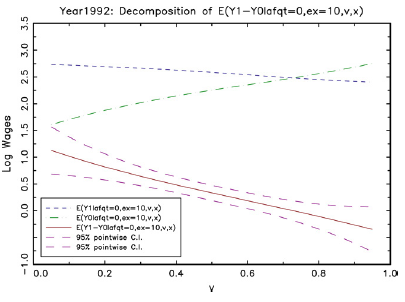
\includegraphics[width=\textwidth]{fig11_1}
\caption{Carneiro, Lee (2009)}
\end{subfigure}
\begin{subfigure}{0.48\textwidth}
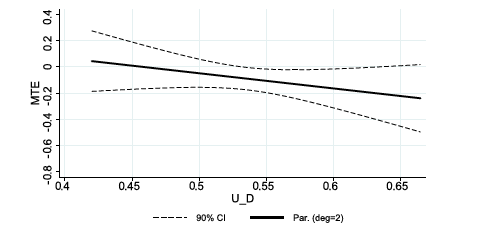
\includegraphics[width=\textwidth]{fig11_2}
\caption{Johnson, Taylor (2019)}
\end{subfigure}
\end{figure}
\end{frame}
%%%%%%%%%%%
\end{document}
